%! Author = adnansiddiquei
%! Date = 19/03/2024

\section{Training the model}\label{sec:q1bc}
\begin{figure}[t]
    \centering
    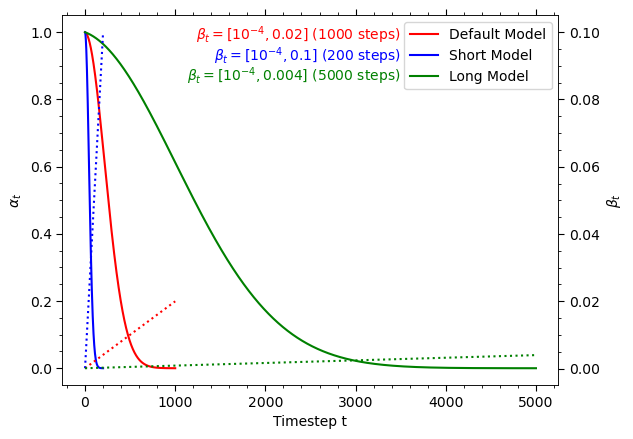
\includegraphics[width=0.8\textwidth]{figures/q1b_noise_schedules}
    \caption{A plot of each noise schedule that was evaluated.
        The dotted lines represent the $\beta_{t}$ values and the solid lines represent the $\alpha_t$ values.}
    \label{fig:q1b_noise_schedules}
\end{figure}

\begin{figure}[t]
    \centering
    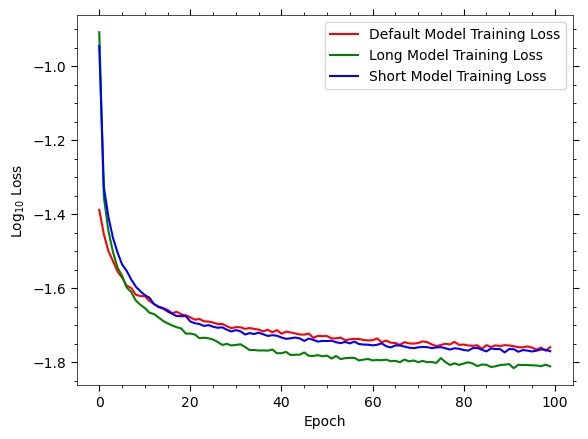
\includegraphics[width=0.8\textwidth]{figures/q1b_training_loss}
    \caption{A plot of the training loss for each model over 100 epochs.}
    \label{fig:q1b_training_loss}
\end{figure}

\begin{figure}
\centering
\begin{subfigure}{0.8\textwidth}
    \centering
    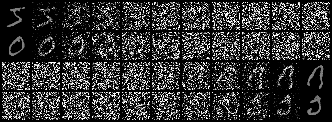
\includegraphics[width=1\textwidth]{./figures/q1b_long_model_nd}
    \caption{The noising (top 2 rows) and denoising (bottom 2 rows) process for the long model, with each column
        representing equal time steps apart (500 time steps).}
    \label{fig:q1b_long_model_nd}
\end{subfigure}%
\hfill
\begin{subfigure}{0.8\textwidth}
    \centering
    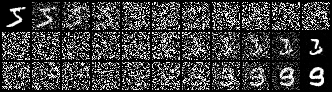
\includegraphics[width=1\textwidth]{./figures/q1b_short_model_nd}
    \caption{The noising (top 2 rows) and denoising (bottom 2 rows) process for the short model, with each column
        representing equal time steps apart (20 time steps).}
    \label{fig:q1b_short_model_nd}
\end{subfigure}
\caption{The noising and denoising process for the long and short models.
    These images illustrate the same process illustrated for the default model in Figure~\eqref{fig:q1a_image_noising}
    and Figure~\eqref{fig:q1a_image_reconstruction}.}
\label{fig:q1b_short_long_model_nd}
\end{figure}

\begin{figure}[t]
    \centering
    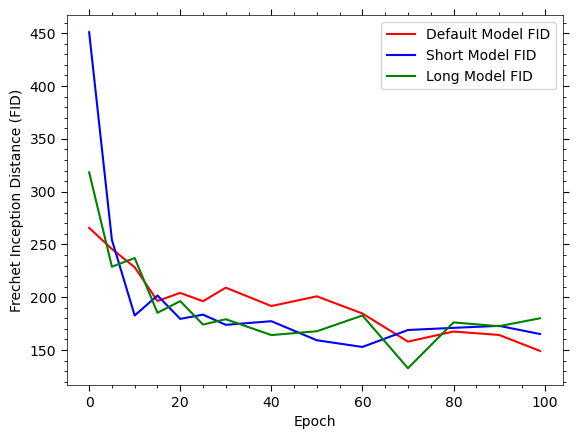
\includegraphics[width=0.8\textwidth]{figures/q1b_fid}
    \caption{A plot of the Frechet Inception Distance (FID) for the generated samples from each model over 100 epochs.
        The FID was calculated using the first 512 samples from the MNIST dataset compared against 32 samples generated
        by each model at varying epochs.}
    \label{fig:q1b_fid}
\end{figure}

This section discusses the training of the DDPM model with varying linear noise schedules.

Three different models were trained, the first model (default model) was trained with the provided noise schedule:
$\beta_{t} = [10^{-4}, 0.02]$ with 1000 steps; the second model (the "long model") was trained with a longer noise schedule:
$\beta_{t} = [10^{-4}, 0.004]$ with 5000 steps which added less noise at each step; and the third model (the "short model")
was trained with a shorter noise schedule: $\beta_{t} = [10^{-4}, 0.1]$ with 200 steps which added more noise at each step.
The number of steps was amended for each model such that the final noise level was the same for each model ($\alpha_{t}$
of the order of $10^{-5}$ at the final time step).
All models were also trained for 100 epochs with a batch size of 128, with the Adams optimiser, a learning rate of
$2 \ times 10^{-4}$ and the same CNN architecture described in Section~\eqref{sec:q1a}.
Figure~\eqref{fig:q1b_noise_schedules} illustrates the noise schedules used for each model, Figure~\eqref{fig:q1b_training_loss}
shows the training loss for each model over 100 epochs, and Figure~\eqref{fig:q1b_short_long_model_nd} illustrates the encoding
and decoding process for the long and short models.
The Frechet Inception Distance (FID) was calculated for each model as the model was trained, as shown in Figure~\eqref{fig:q1b_fid}.
Traditionally, the FID is calculated with the InceptionV3 model, however, given the narrow context of the MNIST dataset,
a simple CNN classifier model was trained on the MNIST dataset and the 1024-length feature vector at
the penultimate layer of this classifier was used to calculate the FID instead.
The MNIST classifier was trained for 7 epochs and attained an accuracy of 99.2\% on the test set, which meant the penultimate
layer was a good feature extractor for the MNIST dataset.
Figure~\eqref{fig:q1b_fid} illustrates that neither model achieved any significant improvement over the others over the
100 epochs, and as expected, the loss curve on Figure~\eqref{fig:q1b_training_loss} matches perfectly with the FID curve.


